\section{Abordagem proposta}

Para determinar os aspectos visuais da manga 'Palmer' mais significativos para a predição de seus atributos de qualidade, foi conduzido um estudo investigativo quanto às variáveis utilizadas na literatura, mostradas na Tabela \ref{tab:artigos_att}. 

Para isto, a técnica utilizada na abordagem proposta foi a \textit{Random Forest}, técnica \textit{ensemble} que combina árvores de decisão para obtenção da variável de saída, o que a torna robusta quanto à presença de ruído nos dados e menos suscetível ao \textit{overfitting} (Chagas et al., 2016). A relação entre as variáveis de entrada e a de saída é modelada através de um conjunto de regras de decisão, construídas por divisões binárias e recursivas dos dados de treinamento de acordo com as variáveis de entrada. Dessa forma, a \textit{Random Forest} é capaz de modelar relacionamentos hierárquicos e não lineares (GUO et al., 2015). As regras de decisão são escolhidas de acordo com a qualidade das predições realizadas, avaliada através da métrica MSE (\textit{Mean Squared Error}), cuja fórmula é mostrada abaixo.

\begin{equation*}
    MSE = \frac{1}{n}\sum_{i=1}^n (y_i - \hat{y}_i)^2
\end{equation*}

Em que $n$ é o número de amostras, $y_i$ é o valor real da variável de saída e $\hat{y}_i$ é o valor previsto para a variável de saída.

A partir da \textit{Random Forest}, é possível obter a importância de cada variável de entrada do modelo, o que permite a seleção das variáveis quando aliada a técnicas como a RFE (\textit{Recursive feature elimination}), que elimina as variáveis de forma recursiva com base em suas importâncias. Em cada iteração deste algoritmo, é treinado o modelo de predição e remove-se a variável menos relevante, até que sobre uma quantidade desejada (Menze et al., 2009), conforme mostra o diagrama da Figura \ref{fig:rf-rfe}. A combinação da RFE com a \textit{Random Forest} forneceu bons resultados nos trabalhos de Granitto et al. (2006) e  Zhou et al. (2014).

\begin{figure}[H]
\centering
    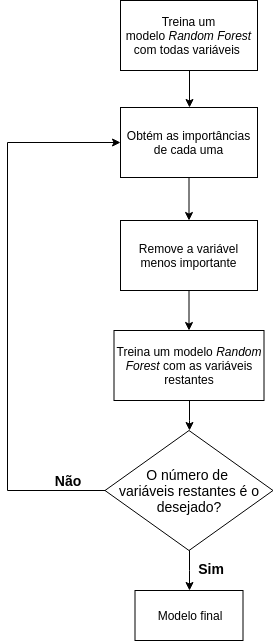
\includegraphics[scale=0.5]{imgs/RF-RFE.png}
    \caption{Diagrama de representação do modelo \textit{Random Forest} aliado à RFE.}\label{fig:abordagem}
\end{figure}

Assim, foram construídos modelos \textit{Random Forest} para cada subconjunto de variáveis identificado nos trabalhos relacionados, que foram codificados conforme a Tabela \ref{tbl:var}. Ademais, foi utilizado o subconjunto que engloba todas as variáveis, a partir do qual foi realizada a seleção de variáveis para redução da dimensionalidade e complexidade do modelo.

\begin{longtable}{l l L{9cm} m{3cm}}
    \caption{Subconjuntos de variáveis obtidos a partir da literatura.}\label{tbl:var}
    \hline
    Id & Nº & Variáveis \\ \hline
    G1 & 1 & Média das intensidades dos pixels no canal L*  \\ \hline
    G2 & 1 & Cor HSV dominante \\ \hline
    G3 & 20 & Média das intensidades RGB na manga inteira, nas regiões apex, equatorial e cume, diferença das médias e gradiente longitudinal \\ \hline
    G4 & 1 & Número de pixels correspondente à manga  \\ \hline
    G5 & 3 & Média das intensidades dos pixels no espaço RGB \\ \hline
    G6 & 6 & Média das intensidades dos pixels no espaço L*a*b* e variáveis fractais (box counting dimension, dilation dimension e correlation dimension)   \\ \hline
    G7 & 1 & Média das intensidades dos pixels no canal Hue \\ \hline
    G8 & 6 & Média das intensidades dos pixels nos espaços HSV e L*a*b* \\ \hline
    G9 & 9 & Média das intensidades dos pixels nos espaços RGB e HSV e taxas R/G, R/B e S/H. \\ \hline
    G10 & 3 & Média das intensidades dos pixels no canal b*, número de pixels e diâmetro \\ \hline
\end{longtable}

Os modelos foram construídos inicialmente para predição da idade das mangas, que variaram entre 35 dias após a floração (DAF) e 20 dias após a colheita (DAC). A partir da determinação do melhor subconjunto de variáveis, foram determinados os atributos de massa, SST, firmeza e acidez titulável. O experimento foi assim conduzido devido à relação entre estes atributos de qualidade e a maturação da fruta, que sofre transformações físicas e químicas durante o processo, resultando em modificações na textura, pigmentação e sabor (Tucker, 1993). Conforme a manga amadurece, são observados o aumento do teor de sólidos solúveis totais e diminuição da acidez titulável e firmeza (Mattoo et al., 1975 e Wills et al., 1981).

Na Figura \ref{fig:abordagem}, é mostrado o diagrama de fluxo do experimento, em que são especificadas as etapas para predição dos atributos de qualidade em mangas 'Palmer'.

\begin{figure}[H]
\centering
    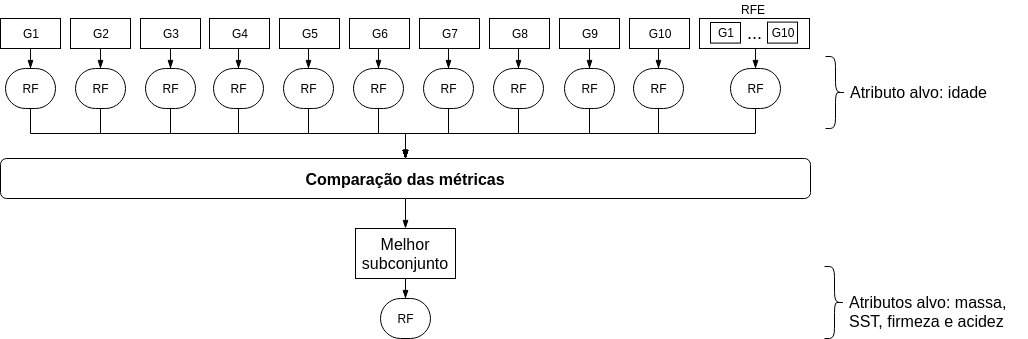
\includegraphics[scale=0.5]{imgs/abordagem_proposta.png}
    \caption{Diagrama de fluxo do experimento.}\label{fig:abordagem}
\end{figure}